	%	\newpage





\section{Fairness Verification of CNF Classifiers with Feature-correlations} 
\label{sec:CNF_feature_correlation}
Existing verifiers such as Justicia focuses mainly on classifiers expressible as a CNF formula. But none of the existing verifiers consider correlation among the features while computing fairness metrics. In this section,  we address fairness verification of CNF-based classifiers with explicit consideration of correlations among features. In particular, we present how to encode a Bayesian network, which captures correlated features, into a SSAT-based formulation that is tailored for verifying CNF classifiers. To this end, we first discuss the basics of SSAT followed by an elaboration of the proposed methodology.



\subsection{Background: Stochastic Boolean Satisfiability (SSAT)}\label{sec:ssat}
Let $ \mathbf{B}  = \{\bool_1, \dots, \bool_m\}  $ be a set of Boolean variables taking assignment in $ \{0,1\}^m $. A \textit{literal} $ l_i $ is a variable $ \bool_i $ or its complement $ \neg \bool_i $. A propositional formula $\phi$ defined over $\mathbf{B}$ is in CNF if $\phi \triangleq \wedge_i C_i $   is  a conjunction of clauses and each clause $ C_i \triangleq \vee_j l_j $ is a disjunction of literals. A CNF formula $ \phi $ is satisfied (called SAT) if there is an assignment $ \sigma $ over $\mathbf{B}$ that evaluates formula $ \phi $ to $ 1 $ (or true)\textemdash at least one literal in each clause is true and all clauses are true. We additionally consider a quantification over each Boolean variable $ B_i $, denoted by $ q_i \in \{\exists, \forall, \R^{p_i}\}$, where $ \exists $ is existential, $ \forall $ is universal and $ \R $ is a randomized quantifier with $ p_i = \Pr[B_i = 1] $. The SSAT problem takes \textit{an ordered set of quantifiers} over  $\mathbf{B}$ and a CNF formula $ \phi $ and computes the \textit{probability of satisfaction} of $ \phi $ given quantifiers.  Formally, a SSAT formula $ \Phi \triangleq (\{q_i\}_{i=1}^{m}, \phi) $ and the SSAT problem computes $ \Pr[\Phi]  \in [0,1]$. The semantics of SSAT formula is in the following.

\begin{enumerate}
	\item $ \Pr[\text{true}] = 1 $,  $ \Pr[\text{false}] = 0 $, 
	\item $ \Pr [\Phi] = \max_{\bool_1} \{\Pr[\Phi|_{\bool_1}], \Pr[\Phi|_{\neg \bool_1}]\}$ if $ \bool_1 $ is existentially quantified ($ \exists $), 
	\item $ \Pr [\Phi] = \min_{\bool_1} \{\Pr[\Phi|_{\bool_1}], \Pr[\Phi|_{\neg \bool_1}]\} $ if $ \bool_1 $ is universally quantified ($ \forall $), 
	\item $ \Pr [\Phi] = p\Pr[\Phi|_{\bool_1}] + (1-p) \Pr[\Phi|_{\neg \bool_1}] $ if $ \bool_1 $ is randomized quantified ($\R^{p}$) with probability $p = \Pr[\bool_1 = 1]$,
\end{enumerate}

In SSAT, we recursively solve for each Boolean variable in $\mathbf{B}$ starting with the first variable $ B_1 $
where $ \Phi|_{\bool_1} $ (resp.\ $ \Phi|_{\neg \bool_1} $) is the SSAT formula with CNF $ \phi $ substituted by an assignment of $ \bool_1 $ as true (resp.\ false) and quantifiers $ \{q_i\}_{i=2}^{m} $. 	

In this paper, we are interested in two specific SSAT formulations: exists-random (ER) SSAT formulas and universal-random (UR) SSAT formulas. In ER-SSAT (resp.\ UR-SSAT), $ \{q_i\} $ is constructed such that  existential (resp.\ universal) quantified variables is followed by randomized quantified variables. For more details on SSAT formulas,  we refer to \cite{ghosh2020justicia,lee2017solving, lee2018solving}.

%This correspondence of existential and universal quantifiers of choice variables with the maximum and minimum probabilities in case of SSAT, motivate us to assign the choice (or sensitive) variables similar quantifiers while computing the maximum and minimum PPVs for linear classifiers.






\subsection{Methodology}
For CNF classifiers~\cite{GMM20}, SSAT is a natural choice as it computes the probability of a CNF formula  given quantifiers of variables\textemdash equivalently, the PPV of a CNF classifier. \cite{ghosh2020justicia} has proposed a SSAT based formulation for verifying a CNF classifier $ \phi_{\hat{Y}} $ with a fundamental limitation of ignoring feature-correlations, which we address now. Let $ \phi_\BN $ be a CNF formula that encodes the Bayesian Network $ \BN $. Following~\cite{ghosh2020justicia}, we discuss an encoding that compute the PPV of the classifier for the most favored sensitive group with additional consideration of features-correlation. Let $\mathbf{Q}$ denote an ordered set of quantifiers over variables in the conjoined CNF $ \phi_{\hat{Y}} \wedge \phi_\BN $. We then construct a SSAT formula $ \Phi =  (\mathbf{Q},  \phi_{\hat{Y}} \wedge \phi_\BN) $ and solve it for computing $ \max_{\mathbf{a}} \Pr[\hat{Y} = 1 | \sensitive = \mathbf{a}] $. For computing $ \min_{\mathbf{a}} \Pr[\hat{Y} = 1 | \sensitive = \mathbf{a}] $ for the least favored group ,only difference is in the construction of $\mathbf{Q}$. We next discuss the construction of both $ \phi_\BN $ and $\mathbf{Q}$.





\paragraph{Encoding a Bayesian Network as a CNF Formula.}\label{sec:BN_to_CNF}
Our goal is to encode the Bayesian network $ \BN = (\graph, \factors) $ into a CNF formula $ \phi_\BN $ such that \textit{the weighted model count} of $ \phi_\BN $ exactly computes a joint probability distribution~\cite{chavira2008probabilistic}.  We note that SSAT does not allow conditional probabilities of randomized quantified variables trivially. Hence, $ \phi_\BN $ contains \textit{additional variables} to capture the conditional probabilities, as discussed next.


Let  $ G = (\mathbf{V}, E) $ where $  $  $ \mathbf{V} \subseteq \nonsensitive \cup \sensitive $ and $ \mathbf{E} \subseteq \mathbf{V} \times \mathbf{V} $. 	For each network variable $ V_i \in \mathbf{V} $, we define a Boolean \textit{indicator}  variable $ \lambda_{V_i} $ such that $ \Pr[\lambda_{V_i}] \triangleq \Pr[V_i] $. We add following constraint in $ \phi_\BN $ to establish the relation between $ \lambda_{V_i} $ and $ V_i $. 
\begin{align}
	\lambda_{V_i} \leftrightarrow V_i,
	\label{eq:indicator_constraint}
\end{align}
Intuitively, both $ \lambda_{V_i} $ and $ V_i $ are either true or false. This constraint can be trivially translated to clauses in CNF using the equivalence rule $ a \leftrightarrow b\equiv (\neg a \vee b)  \wedge (a \vee \neg a) $ for Boolean variables $ a, b$.

We now show encoding of conditional probabilities induced by parameter $ \theta $. Let $ V_i \in  \mathbf{V}  $  be a vertex in $ G $ where $ \parent(V_i) \ne \emptyset $ be $ V_i $'s parents and $ |\parent(V_i)| = k $. Additionally, let $ v $ and $ \mathbf{u} \triangleq [u_1,.., u_k] $ be an assignment of  $ V_i $ and $ \parent(V_i)  $, respectively.  To encode $ \Pr[V_i = v| \parent(V_i) = \mathbf{u}]$, we introduce auxiliary variable $ \lambda_{v,\mathbf{u}} $ and add following constraints in $ \phi_{\BN} $.
\begin{align}
	\lambda_{v,\mathbf{u}}  \wedge \bigwedge_{j=1}^{k} \lambda_{u_j} \rightarrow \lambda_v
	\label{eq:factor_pos}
\end{align}
\begin{align}
	\neg \lambda_{v,\mathbf{u}}  \wedge \bigwedge_{j=1}^{k} \lambda_{u_j} \rightarrow \neg \lambda_v
	\label{eq:factor_neg}
\end{align}

where $ \lambda_v \equiv \lambda_{V_i} $. Moreover, $ \lambda_{u_j} $ is the indicator variable corresponding to the $ j^\text{th} $ parent in $ \parent(V_i) $. In the above two constraints,	for a fixed assignment $ \mathbf{u} $ of parents $ \parent(V_i) $, both $ \lambda_v $ and $ \lambda_{v,\mathbf{u}} $ are either true or false.  Hence, these two constraints encode the conditional probability of $ V_i = v $ given $ \parent(V_i) = \mathbf{u} $ using $ \Pr[\lambda_{v,\mathbf{u}}] = \Pr[V_i = v| \parent(V_i) = \mathbf{u}]$. Both constraints can be translated to CNF clauses trivially. For example, Eq.~\ref{eq:factor_pos} is translated as $ \neg \lambda_{v,\mathbf{u}}  \vee \bigvee_{j=1}^{k} \neg \lambda_{u_j} \vee \lambda_v $. We next analyze the complexity of $ \phi_\BN $ in terms of the number of variables and clauses.

\begin{lemma}
	For a Bayesian network $ \BN = (\graph, \factors) $ defined over $ n $ Boolean network variables, the encoded CNF formula $ \phi_\BN $ has $ n + |\factors| $  variables and $ 2(n + |\factors|) $ clauses. 
\end{lemma}
\begin{proof}
	Since the DAG in the Bayesian network has $ n $ vertices, we consider $ n $ indicator variables. Moreover, for encoding conditional probabilities, we consider $ |\theta| $ auxiliary variables where parameter $ \theta $ denotes the number of distinct conditional probabilities in the network. Hence, total variables in $ \phi_\BN $ is $ n + |\factors|  $.
	
	According to Eq.~\eqref{eq:indicator_constraint},~\eqref{eq:factor_pos},~\eqref{eq:factor_neg}, there are $2( n + |\theta|) $ clauses in $ \phi_\BN $ as discussed in Section~\ref{sec:BN_to_CNF}.
	
	
\end{proof}

\begin{figure}[!t]
	\begin{center}
		\subfloat[]{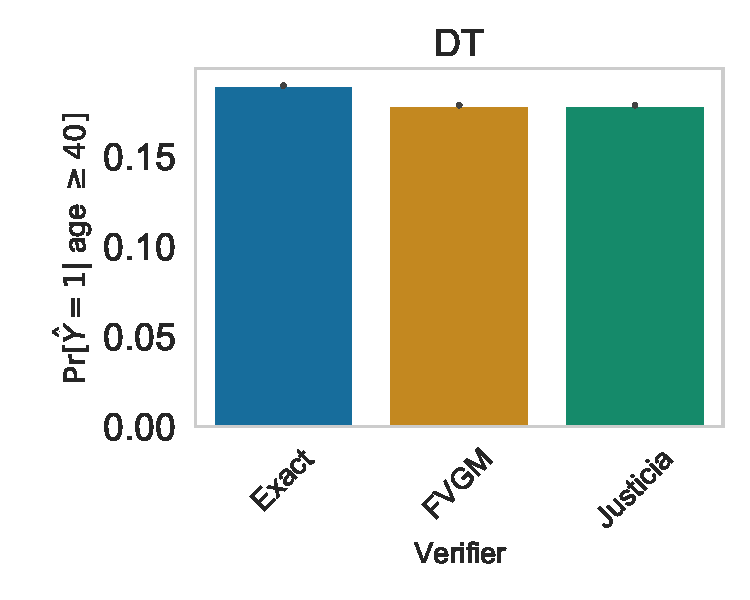
\includegraphics[scale=0.33]{figures/sanity_ppv_max_PPV_DT}}
		\subfloat[]{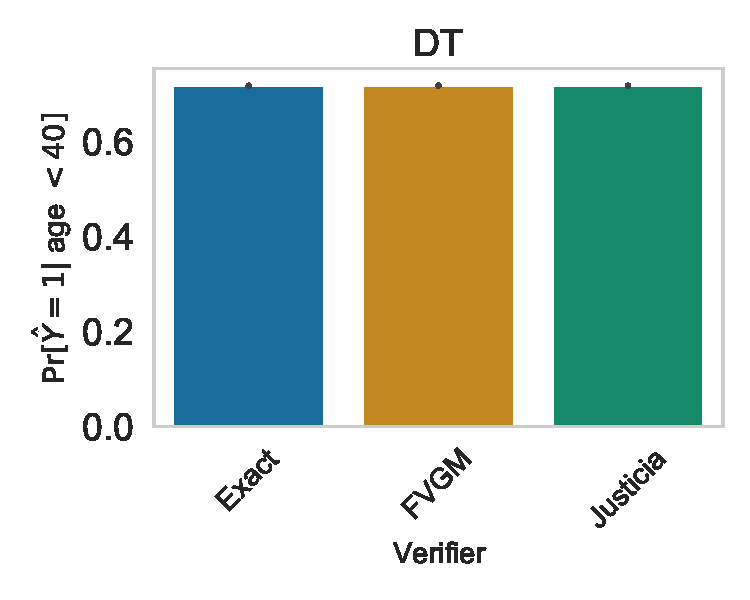
\includegraphics[scale=0.33]{figures/sanity_ppv_min_PPV_DT}}\\
		\subfloat[]{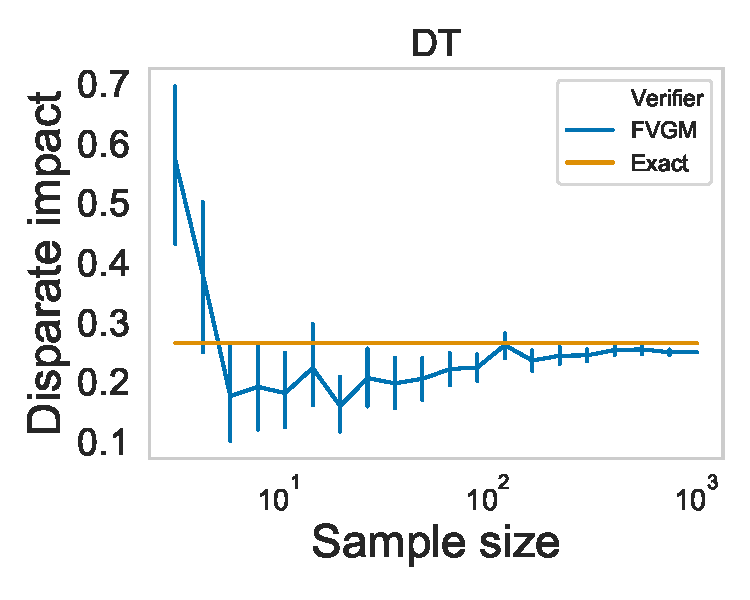
\includegraphics[scale=0.33]{figures/sanity_sample_size_DI_DT}}
		\subfloat[]{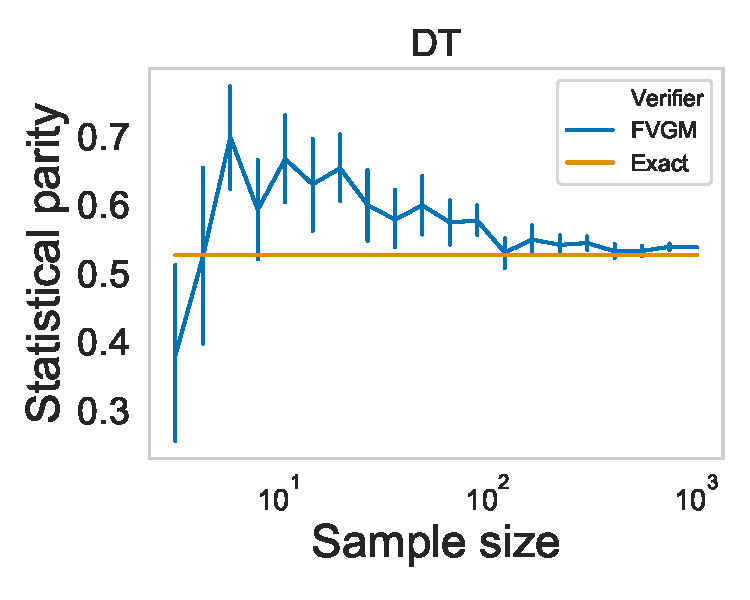
\includegraphics[scale=0.33]{figures/sanity_sample_size_SPD_DT}}
		
		
	\end{center}
	
	\caption{
		Computing PPV of Decision Tree (DT) classifiers using {\framework} and Justicia. {\framework} incorporates correlated features represented as a Bayesian network in Figure~\ref{fig:synthetic_bn}. We also present the effect of sample size on different fairness metrics such as DI and SP for DT classifier. }
	\label{fig:synthetic_results}
\end{figure}

\paragraph{Constructing Quantifiers $ \mathbf{Q} $.}
We now discuss the ordered set of quantifiers for a SSAT formula containing CNF $ \phi_{\hat{Y}} \wedge \phi_\BN $\textemdash the solution of which constitutes the maximum (minimum) PPV of a CNF classifier. $ \phi_{\hat{Y}} \wedge \phi_\BN $ contains four different variables : (i) sensitive variables $ \sensitive $, (ii) non-sensitive variables $ \nonsensitive $, (iii) indicator variables $  \lambda_{V_i} $, and (iv) auxiliary variables $ \lambda_{v,\mathbf{u}} $. Among them, (iii) and (iv) are associated with $ \phi_\BN $ and the rest for $ \phi_{\hat{Y}} $. For computing the maximum PPV of the classifier, we construct  an exists-random-exists (ERE) SSAT formula with quantifiers $\mathbf{Q}$ as follows: we set sensitive features $ \sensitive $ with existential quantifiers in the beginning of $ \mathbf{Q} $ followed by $  \lambda_{V_i}, \lambda_{v,\mathbf{u}} $ and $ X_j \in \nonsensitive \setminus \mathbf{V} $ with randomized quantifiers. Since sensitive variables are existentially quantified\textemdash similar to stochastic subset-sum problem\textemdash the solution of SSAT formula is maximized.
Finally, remaining variables appearing in the Bayesian network such as $ X_i \in \mathbf{V} $ are existentially quantified in $\mathbf{Q}$ as their assignment is fixed by indicator variables $ \lambda_{V_i} $. In contrast, for computing the minimum PPV of the classifier, we consider an universal-random-exists (URE) SSAT formula  where we set sensitive features $ \sensitive $ as universal quantifiers with all other quantifiers remaining same.


\iffalse
\subsection{Verifying Classifiers with Non-Boolean Features} {\framework} can verify beyond non-Boolean features. For binary decision tree classifiers, real-valued features are discretized in each node of the tree by comparing the feature against a constant threshold. Thus, each node constitutes a Boolean feature and the tree itself forms a CNF formula, as shown by~\cite{ghosh2020justicia}.
\fi





